\documentclass[12pt]{article} 

%?? paths

%?? packages 
\usepackage{setspace,geometry,fancyvrb,rotating} 
\usepackage{marginnote,datetime,enumitem} 
\usepackage{titlesec,indentfirst} 
\usepackage{amsmath,amsfonts,amssymb,amsthm,mathtools} 
\usepackage{threeparttable,booktabs,adjustbox} 
\usepackage{graphicx,epstopdf,float,soul,subfig} 
\usepackage[toc,page]{appendix} 
\usdate

%?? page setup 
\geometry{scale=0.8} 
\titleformat{\paragraph}[runin]{\itshape}{}{}{}[.] 
\titlelabel{\thetitle.\;} 
\setlength{\parindent}{10pt} 
\setlength{\parskip}{10pt} 
\usepackage{Alegreya} 
\usepackage[T1]{fontenc}
\usepackage{notomath}
\usepackage[T1]{fontenc}
% \usepackage{fourier} % Favorite Font

%?? bibliography 
\usepackage{natbib,fancybox,url,xcolor} 
\definecolor{MyBlue}{rgb}{0,0.2,0.6} 
\definecolor{MyRed}{rgb}{0.4,0,0.1} 
\definecolor{MyGreen}{rgb}{0,0.4,0} 
\definecolor{MyPink}{HTML}{E50379} 
\definecolor{MyOrange}{HTML}{CC5500} 
\definecolor{MyPurple}{HTML}{BF40BF}
\newcommand{\highlightR}[1]{{\emph{\color{MyRed}{#1}}}} 
\newcommand{\highlightB}[1]{{\emph{\color{MyBlue}{#1}}}} 
\newcommand{\highlightP}[1]{{\emph{\color{MyPink}{#1}}}} 
\newcommand{\highlightO}[1]{{\emph{\color{MyOrange}{#1}}}}
\newcommand{\highlightPP}[1]{{{\color{MyPurple}{#1}}}}
\usepackage[bookmarks=true,bookmarksnumbered=true,colorlinks=true,linkcolor=MyGreen,citecolor=MyGreen,filecolor=MyBlue,urlcolor=MyGreen]{hyperref} 
\bibliographystyle{econ}

%?? math and theorem environment 
\theoremstyle{definition} 
\newtheorem{assumption}{Assumption} 
\newtheorem{definition}{Definition} 
\newtheorem{theorem}{Theorem} 
\newtheorem{proposition}{Proposition} 
\newtheorem{lemma}{Lemma} 
\newtheorem{example}{Example} 
\newtheorem{corollary}[theorem]{Corollary} 
\usepackage{mathtools} 
\usepackage{makecell}

\begin{document} 

%??%??%??%??%??%??%??%??%??%??%??%??%??%??%??%??%??%??%??%??%??%?? 
%?? title 
%??%??%??%??%??%??%??%??%??%??%??%??%??%??%??%??%??%??%??%??%??%??

\title{\bf 2025-03-19 Code Review Task} 
\author{Wenzhi Wang} 
\date{\today} 
\maketitle 

\section{Overview of the task}

The task is to review codes stored in the ``01Main'' folder, which can reproduce all tables and figures in Virginia's job market paper. However, it does \highlightP{not} simply require you to check that they can run without errors and can produce the same results as in the paper. \highlightP{Instead, it requires you to check the codes can produce something that makes sense, that fits the description in the paper.} Thus, a thorough understanding of the paper and attention to details are crucial.

\subsection{Introduction to the project folder}

The folder tree of this project is in Figure \ref{ProjectTree}, which can also be seen as in the ``0000Master.do'' file in the ``Dofiles/01Main'' folder. 
\begin{figure}[H]
    \noindent\caption{Folder tree of the project}
    \vspace{-10pt}
    \begin{center}
        \resizebox{0.33\textwidth}{!}{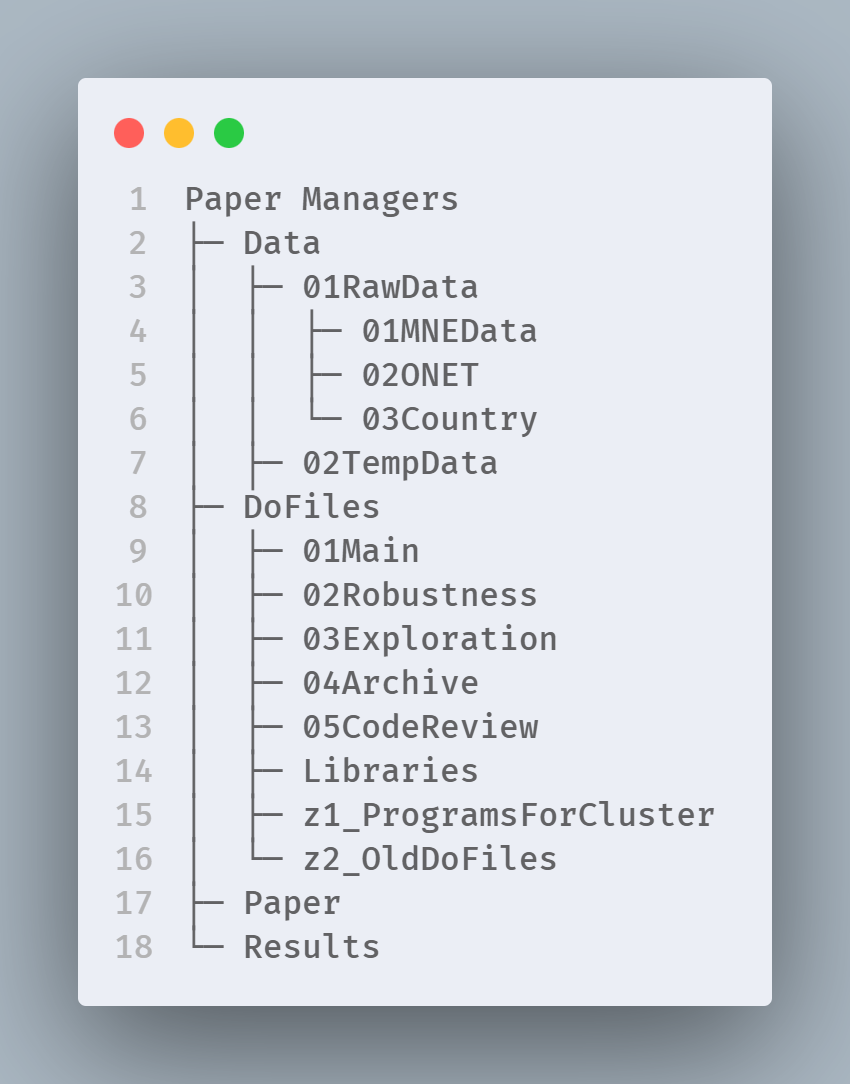
\includegraphics{ProjectTree.png}}
        \label{ProjectTree}
    \end{center}
\end{figure}
It is important to set up these same folders in the beginning, which is a necessary requirement in the paths specification step of the ``Dofiles/01Main/0000Master.do'' file.

The code review task requires you to focus on the following two folders:
\begin{itemize}[topsep=0pt, leftmargin=20pt, itemsep=0pt]
	\setlength{\parskip}{10pt} 
	\item ``DoFiles/01Main'' folder contains the main do files, and you will access to them through GitHub repository \href{https://github.com/wenzhi-econ/V-Managers}{https://github.com/wenzhi-econ/V-Managers}.
	\item ``Data/01RawData'' folder contains all necessary raw data, and you will access to these datasets through Chicago Booth's computing cluster \href{https://hpc-docs.chicagobooth.edu/intro.html}{(link here)}\footnote{The raw data contains proprietary HR records from a multinational firm, so you \highlightP{must not} share the data with anyone. An additional ``no-share'' agreement will be signed later. Also, you will access the Mercury through my pre-doc's account to save unnecessary administrative costs to connect you to the cluster, so please do not do anything that may jeopardize the security of his account. Apart from accessing the datasets, you will also need to run event studies on Mercury, after maybe testing the codes on a 1\% sample locally on your laptop.}.
\end{itemize}

\subsection{Introduction to the ``DoFiles/01Main'' folder}

The ``DoFiles/01Main/\_Description.md'' file contains some introductory information for this folder. In particular, it briefly talks about different goals of do files whose names start with different numbers, and contains a mapping between the do files and the tables/figures in the paper. The mapping is also provided in Table \ref{tab_mapping}. Therefore, it is helpful to go through this file before starting to review and modify the original codes.

The ``DoFiles/01Main/0000Master.do'' file is the master do file in the folder, and should be the starting point of this task. It has the following utilities:
\begin{itemize}[topsep=0pt, leftmargin=20pt, itemsep=0pt]
	\setlength{\parskip}{10pt} 
	\item default Stata setups, e.g., version control;
	\item paths specification for the project, which needs to be adapted to your own local paths;
	\item installation of necessary community packages to a local directory ``DoFiles/Libraries'' and guarantee to use these local ado files (Line 86 should be uncommented in your first execution to install these packages);
	\item figure scheme specification; and most importantly,
	\item do files for producing results in the table (they are ordered in this master do file by their importance and easiness to run).
\end{itemize}

In each do file in the ``DoFiles/01Main'' folder, the comments in the beginning will provide some necessary information about the corresponding file. For example, in ``DoFiles/01Main/0301\_01.do,'' it contains the purpose of the do file, some notes on the specification of the event study, necessary input files, and output of the do file. These comments may be helpful in some circumstances for you to understand the original codes. In Section \ref{sec_standards}, there are some standards to follow when you modify the do files, and write your own do files.

\subsection{Recommended procedures to approach the task}

\begin{enumerate}[topsep=0pt, leftmargin=20pt, itemsep=0pt, label=(\arabic*)]
	\setlength{\parskip}{10pt} 
	\item Read the paper carefully. Two versions of the paper are provided. 
	\begin{itemize}[topsep=0pt, leftmargin=20pt, itemsep=0pt]
        \setlength{\parskip}{10pt} 
        \item The first one is the ``20241002'' version, which is self-contained and complete. However, the paper is restructured in 2025, with some results deleted and some new results added. 
        \item The second version is the ``20250320'' version, which contains the most up-to-date results generated from the codes you are asked to review. However, it is still a work in progress, so some explanation and description may be missing, and there are a lot of comments and notes in the main text, which may damage the readability of the paper.
        \item You should start with the first version to get a general understanding of the paper, and then proceed to the second version to get a sense of the most up-to-date results, and to start the code review task with the most recent results in mind.
    \end{itemize}
	\item Check the functionality of the original codes.
	\begin{itemize}[topsep=0pt, leftmargin=22pt, itemsep=0pt]
        \setlength{\parskip}{10pt} 
        \item In this step, it is better to simply run the codes without any modification.
        \item There is no need to run all do files in this step, as some analysis involves some tricky variable construction procedures or extremely long execution time, and these niche parts (which may be likely to appear only once) are not key for original codes.
        \item A recommended order is as follows:
        \begin{itemize}[topsep=0pt, leftmargin=20pt, itemsep=0pt]
            \setlength{\parskip}{10pt} 
            \item Start with the data cleaning do files, i.e., do files whose names start with ``01.'' 
            
            Ignore maybe ``0105, 0106'', or even two ``0107'' files in the beginning, as they are not the most important parts of the data cleaning process.
            \item Continue with some do files used to generate summary statistics results in the paper, e.g., ``0401, 0402, 0403, 0601, 0602, 0701, 0702, 0703.''
            \item Proceed to do files for event studies. Some of them require the cluster, while others can be run locally. 
            
            For the latter, you can try to first get familiar with ``0303, 0305''. 
            
            For the former, it is better to run only the ``0301\_01'' do file (along with the do files ``0201, 0202, 0203'' that store necessary Stata programs for this file) in this step. This step serves three goals: (1) to have a basic understanding of the original codes for generating event study results, e.g., generating ``event $\times$ relative time period'' dummies and storing them as global macros; (2) to have a basic understanding of the quarterly aggregation procedures, which transforms the raw monthly level coefficients into quarter level; and (3) to know how to use Mercury to submut a task, extract the results, etc.
        \end{itemize}
    \end{itemize}
	\item Start the code review task using the workflow introduced in Section \ref{sec_workflow}.
	\begin{itemize}[topsep=0pt, leftmargin=22pt, itemsep=0pt]
        \setlength{\parskip}{10pt} 
        \item Start with the data cleaning do files.
        \item Continue with do files for generating event study results.
        \item Check codes for generating other tables and figures in the paper.
        \item Finally, check codes for producing other statistics cited in the paper (if time permits).
    \end{itemize}
\end{enumerate}



\section{GitHub workflow: Upload, get reviewed, and re-upload} \label{sec_workflow}

\begin{enumerate}[topsep=0pt, leftmargin=20pt, itemsep=0pt, label=(Step \arabic*)]
	\setlength{\parskip}{10pt} 
	\item Create your own GitHub account.
	
	\item Go to link here \href{https://github.com/wenzhi-econ/V-Managers}{https://github.com/wenzhi-econ/V-Managers} and select \highlightPP{Fork} on the top right corner to create a copy of the repository.
	
	\item Download the baseline do files to your own laptop, and make changes to the do files, according to the standards outlined in Section \ref{sec_standards}.
	
    After writing codes locally, upload the new or modified do files to the corresponding folder in your forked repository. In this step, you need to \highlightPP{commit changes}, and make sure your commits have a clear and meaningful message.
	
	\item \highlightPP{Create a new branch} with an intuitive name (such as ``data\_cleaning,'' ``descriptive\_stats''), and upload the modified do files to the new branch.
	
	\item Select the Contribute botton to \highlightPP{start a pull request} to the original repository. 
    
    In the pull request, submit the corresponding task report in pdf, and briefly describe the issues you found in the code review task using Markdown syntax.
	\item After the codes are reviewed, and the report is discussed, modify the do files according to the comments, and upload the modified do files to the same branch. This will automatically \highlightPP{update the pull request}.
	
	\item When all issues you found are resolved, the modified do files will be merged to the original repository. Then go back to (Step 4) and create a new branch for the next part of the code review task. {The old branch can then be deleted after the pull request is merged.}
\end{enumerate}

If you have doublt in any of the steps, we can have a Zoom meeting to discuss the issues. There is no need to spend too much time on the workflow itself (e.g., to be a Git or GitHub master), as it is simply a collaboration tool to facilitate the code review task. 

\section{Do files and task reports} \label{sec_standards}

This task involves with modifying the original do files, and writing your own do files. \highlightP{A general principle is that changes to the original do files should be used for illustration, and actual changes should be stored in your own do files, and uploaded to the ``DoFiles/05CodeReview'' folder in the repository.}

\begin{itemize}[topsep=0pt, leftmargin=20pt, itemsep=0pt]
	\setlength{\parskip}{10pt} 

    \item \highlightP{Changes in original do files} are used to illustrate the issues you found in the code review process. 
    
    For example, if you find a $\mathtt{generate}$ command is wrong because missing values are not considered, then you should keep the original codes and add your proposed changes in the same do file. The post-modification do file need not to be executed successfully -- they are simply used to illustrate what issues you found, so that I can review them when you submit the pull request.
    
    You should mark any issues you found in the original do files, and provide a brief explanation in the do file. For one issue that appears multiple times, it is ok to mark it only once.

    \item \highlightP{Your own do files} should be stored in the ``DoFiles/05CodeReview'' folder in the repository. They should be free of errors, and are used to generate results in your task report.
    
    The following are some standards for writing your own do files:
    \begin{itemize}[topsep=0pt, leftmargin=22pt, itemsep=0pt]
        \setlength{\parskip}{10pt} 
        \item They should have a consistent naming patterns with the original do files. 
        \item In the beginning of each do file, you should provide a brief explanation of the purpose of the do file, the necessary input files, and the output in comments. Make sure your name and the date are also included.
        \item A single do file should not be too long, and should be split into multiple code blocks based on their logical structure. The specific commenting structure for splitting the do files should be consistent with the original do files.
        \item Do \highlightP{not} replace the original datasets (raw MNE HR datasets, and also the intermediary datasets generated by original do files) in your own codes. It is better if your datasets share a similar name with the original datasets, but not the same, so that I can compare the original datasets with yours when necessary. 
        
        A related issue is that do \highlightP{not} upload any datasets to the GitHub repository. (You will be not allowed to upload them due to the size limit of a GitHub repository.) In general, if there are some intermediary datasets necessary for your task report, I will run your do files to generate it personally. 
    \end{itemize}
    
    \item In the \highlightP{task report}, you should write down a summary of the issues you have found in the original do files, the explanation of the issues, and how you resolve them in your own do files. It is better if you can compare the different results generated by the original do files and your own do files. The task reports should be stored in the ``05CodeReview/0500\_02'' folder to keep track of your work.
\end{itemize}

\section{Mercury workflow: Access files, and submit tasks}

Accessing the Mercury cluster is necessary for running the event studies, as they will take an extremely long time to run on your own laptop. In this code review task, you will connect to Mercury through my pre-doc's account. 

The general introduction of the cluster is \href{https://hpc-docs.chicagobooth.edu/intro.html}{here}. It is helpful to go through the entire tuturial to get your self familiar with some basic concepts and procedures in the cluster. For this task, you need to interact with the cluster in the following three ways:
\begin{enumerate}[topsep=0pt, leftmargin=20pt, itemsep=0pt, label=(\alph*)]
	\setlength{\parskip}{10pt} 
    \item Connecting to Mercury -- the reference is \href{https://hpc-docs.chicagobooth.edu/connecting.html#}{here}.
	\item Exchanging files -- the reference is \href{https://hpc-docs.chicagobooth.edu/accessing.html}{here}. In particular, I use ``Filezilla'' application to transfer files between my laptop and Mercury.
	\item Submitting tasks -- the reference is \href{https://hpc-docs.chicagobooth.edu/running.html}{here}. The ``Interactive Login'' part is not relevant, as you will not run the codes interactively. Instead, you will submit a batch job to run the codes.
    Specifically for Stata, \href{https://hpc-docs.chicagobooth.edu/Stata/stata.html#batch-mode}{this} teaches you how to structure a .sh file to be submitted.
\end{enumerate}

% \highlightR{To VM: A tricky thing is that to access Mercury, an additional requirement is to have a Chicago VPN connection if the RA is not on a UChicago campus network. This requires my own password that linkd to my email account and all other resources. So this task can be really tricky if the RA is not a Chicago student.}

In the ``DoFiles/z1\_ProgramsForCluster'' folder, there are two examples. Further instructions will be provided if you decide to accept the code review task.

\begin{table}[H]
	\centering
	\caption{Mapping from output to script file(s)}
    \resizebox{1\textwidth}{!}{
    \begin{tabular}{lr}
        \toprule \toprule 
        Output in paper & File(s)  \\ 
        \toprule
        \multicolumn{2}{l}{\emph{Figures in the main text}} \\
        \toprule
        Figure Ia & 0601DescriptiveFigure\_WLAgainstTenureDist.do \\
        Figure Ib & 0602DescriptiveFigure\_TenureAtPromDist.do \\
        Figure IIa, IIb & 0301\_01TwoMainOutcomesInEventStudies.do \\
        Figure IIc, IId & 0301\_06ExitOutcomes\_InvolAndVol.do \\
        Figure III & 0302Decomp\_TransferSJC.do \\
        Figure IVa, IVb, IVc & 0301\_02PayOutcomesInEventStudies.do \\
        Figure IVd & 0301\_03WLPromotionsInEventStudies.do \\
        Figure V & 0304FactoryLevel\_ProductivityAndCostOutcomes.do \\
        Figure VIa, VIb & 0301\_01TwoMainOutcomesInEventStudies.do \\
        Figure VIc, VId & 0301\_06ExitOutcomes\_InvolAndVol.do \\
        Figure VII & 0301\_01TwoMainOutcomesInEventStudies.do \\
        \toprule
        \multicolumn{2}{l}{\emph{Tables in the main text}} \\
        \toprule
        Table I & 0401SummaryStatistics\_ObsSize.do \\
        Table II & 0402SummaryStatistics\_WholeSample.do \\
        Table III & 0403SummaryStatistics\_MngrHvsL\_FullMngrSample.do \\
        Table IV & 0404ProdResultsConditionalOnLateralAndVerticalMoves.do \\
        Table V & 0303FourMainOutcomes\_Heterogeneity.do \\
        \toprule
        \multicolumn{2}{l}{\emph{Appendix figures}} \\
        \toprule
        Figure A.3 & 0701DescriptiveFigure\_WLYearProfiles.do \\
        Figure A.5 & 0702DescriptiveFigure\_PayRelatedVarsCorrelation.do \\
        Figure A.6 & 0703DescriptiveFigure\_ShareMoversAcrossSubFuncs.do \\
        Figure A.7a & 0301\_05ProbLateralTransferInEventStudies.do \\
        Figure A.7b & 0301\_04ONETTaskDistance.do \\
        Figure A.8 & 0705\_01SkillTransferHeatmap\_LtoLvsLtoH.do, 0705\_02OccTaskTransitionHeatMap.py \\
        Figure A.9a, A.9b & 0303\_04Robustness\_CohortDynamics\_LtoHvsLtoL.do \\
        Figure A.9c, A.9d & 0303\_05Robustness\_CohortDynamics\_HtoLvsHtoH.do \\
        Figure A.10a, A.10b & 0303\_01Robustness\_SingleCohortYear.do \\
        Figure A.10c, A.10d & 0303\_02Robustness\_NewHires.do \\
        Figure A.10e, A.10f & 0303\_03Robustness\_Poisson.do \\
        Figure A.11 & 0704\_01SkillsDescriptionLDA.py, 0704\_02SkillsComparison.do \\
        Figure A.12 & 0305TeamLevel\_InequalityDynamics.do \\
        \toprule
        \multicolumn{2}{l}{\emph{Appendix tables}} \\
        \toprule
        Table B.1 & 0502EndogenousMobilityChecks\_toH.do \\
        Table B.2 & 0503EndogenousMobilityChecks\_toHVStoL.do \\
        Table B.3 & 0501HFIsNotAnLaggingIndicator.do \\
        Table B.4 & 0504TimeUse\_MngrHvsL.do \\
        Table B.5 & 0505ActiveLearning\_MngrHVsL.do \\
        Table B.6 & 0506FlexibleProjects\_MngrHVsL.do \\
        Table B.7 & 0507\_01Network\_WorkInfo.do, 0507\_02Network\_ColleagueInfo.do, 0507\_03\_Network\_Regressions.do \\ 
        Table B.8 & 0508JobCreation.do \\
        \bottomrule
    \end{tabular}
    }
    \label{tab_mapping}
\end{table}

\end{document}